\section{Descripción técnica-conceptual del proyecto a realizar}
\label{sec:descripcion}

\quad El presente proyecto presenta una solución al problema que tiene el curso de \empclientename\hspace{1px} quienes carecen del equipo necesario para poder mantener las muestras de bacterias que requieren para sus experimentos, debido a que las mismas deben conservarse a una temperatura determinada para el correcto desarrollo del proceso.

\quad Para solucionarlo se construirá una conservadora con un sistema de control de temperatura, la cual se podrá controlar mediante una aplicación para teléfonos celulares.

\quad La conservadora constará de un recipiente con forma de cubo aislado térmicamente. La temperatura interior del mismo será medida por un sensor de temperatura y regulada a partir de dos celdas peltier governadas por un microprosesador ESP8266.
\newline
\begin{figure}[h]
  \centering
  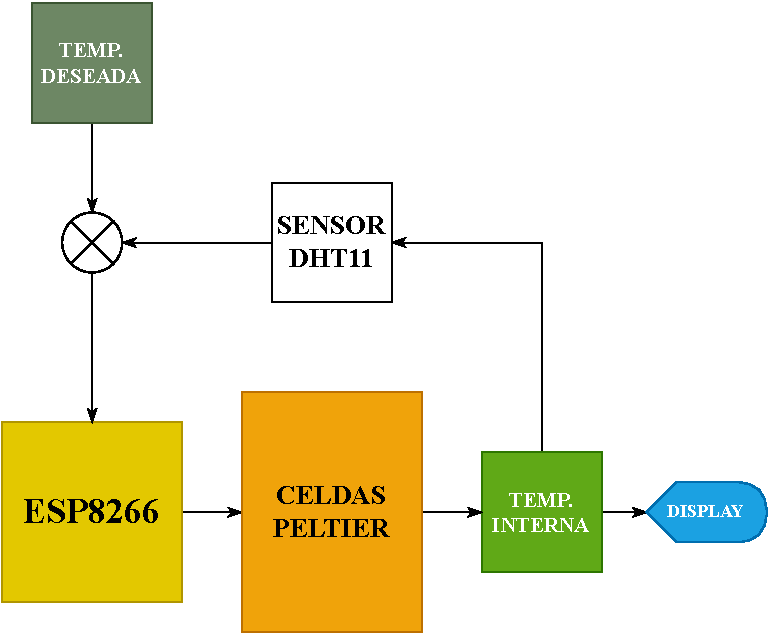
\includegraphics[width=0.9\textwidth]{./Figuras/diagrama.pdf}
  \caption{Diagrama en bloques del funcionamiento de la conservadora}
  \label{fig:diagrama}
\end{figure}
\quad La figura \ref{fig:diagrama} Muestra el diagrama en bloques del sistema de la conservadora.
\pagebreak